\documentclass[a4paper]{article}
\usepackage[warn]{mathtext}
\usepackage[utf8]{inputenc}
\usepackage[T2A]{fontenc}
\usepackage[english,russian]{babel}
\usepackage{booktabs}
\usepackage{multicol}
\usepackage{fancyhdr}
\usepackage{graphicx}
\usepackage{microtype}
\usepackage{wrapfig}
\usepackage{amsmath}
\usepackage{floatflt}
\usepackage{geometry} \geometry{verbose,a4paper,tmargin=2cm,bmargin=2cm,lmargin=1.5cm,rmargin=1.5cm}
\usepackage{float}
\usepackage{amssymb}
\usepackage{caption}
\usepackage{epsfig}
\usepackage{newunicodechar}

\begin{document}

\graphicspath{ {pictures/} }
\begin{center}
    {\scshape\Large Экзамен по дисциплине \par <<Электронные своства твердых тел>>} \par

    \

    {\huge\bfseries Билет № 24} \par 

    \

    {\large Яромир Водзяновский Б04-855а}
\end{center}

\

\

\begin{enumerate}
    \item \textbf{Пояснить возникновение плазменных колебаний с указанием их собственной частоты.} \par 
    \textit{Плазменная частота} - частота собственных продольных колебаний пространственного заряда (ленгмюровских колебаний) в однородной плазме в отсутствие магнитного поля. В пренебрежении движением ионов плазменная частота электронного газа равна (в системе СГС): \par 
    $$\omega_{pe} = \sqrt{\frac{4 \pi n_e e^2}{m_e}} = 5.6415 \cdot 10^4 \sqrt{n_e} \; \frac{рад}{c}$$
    Предположим, что дебаевская длина достаточно велика и для плазмы характерно дальнодействие кулоновских сил, благодаря чему она может рассматриваться как упругая среда. Если группу электронов в плазме сдвинуть из их равновесного положения (тяжёлые ионы считаем неподвижными), 
    то на них будет действовать электростатическая возвращающая сила, что и приводит к колебаниям.

    \item \textbf{Проиллюстрировать процесс Оже-генерации. Почему энергия первичного (затравочного) носителя всегда больше ширины запрещенной зоны? } \par 
    \textit{Оже-генерация} - механизм генерации, противоположный Оже - рекомбинации. Ударная генерация осуществляется дырками или электронами полупроводника, которые под действием приложенного к полупроводнику электрического 
    поля приобретают энергию, достаточную для образования пары носителей. При взаимодействии таких электронов или дырок с атомами матрицы кристалла, возможна передача атому энергии, достаточной для разрыва ковалентной связи и образования пары. \par 
    Энергия затравочного электрона должна быть больше ширины запрещенной зоны в связи с телповыми потерями. Оже-электрону необходима энергия > $E_{gap}$, так как они могут возбуждаться из уровней ниже, чем валентная зона.

    \begin{figure}[H]
        \begin{center}
            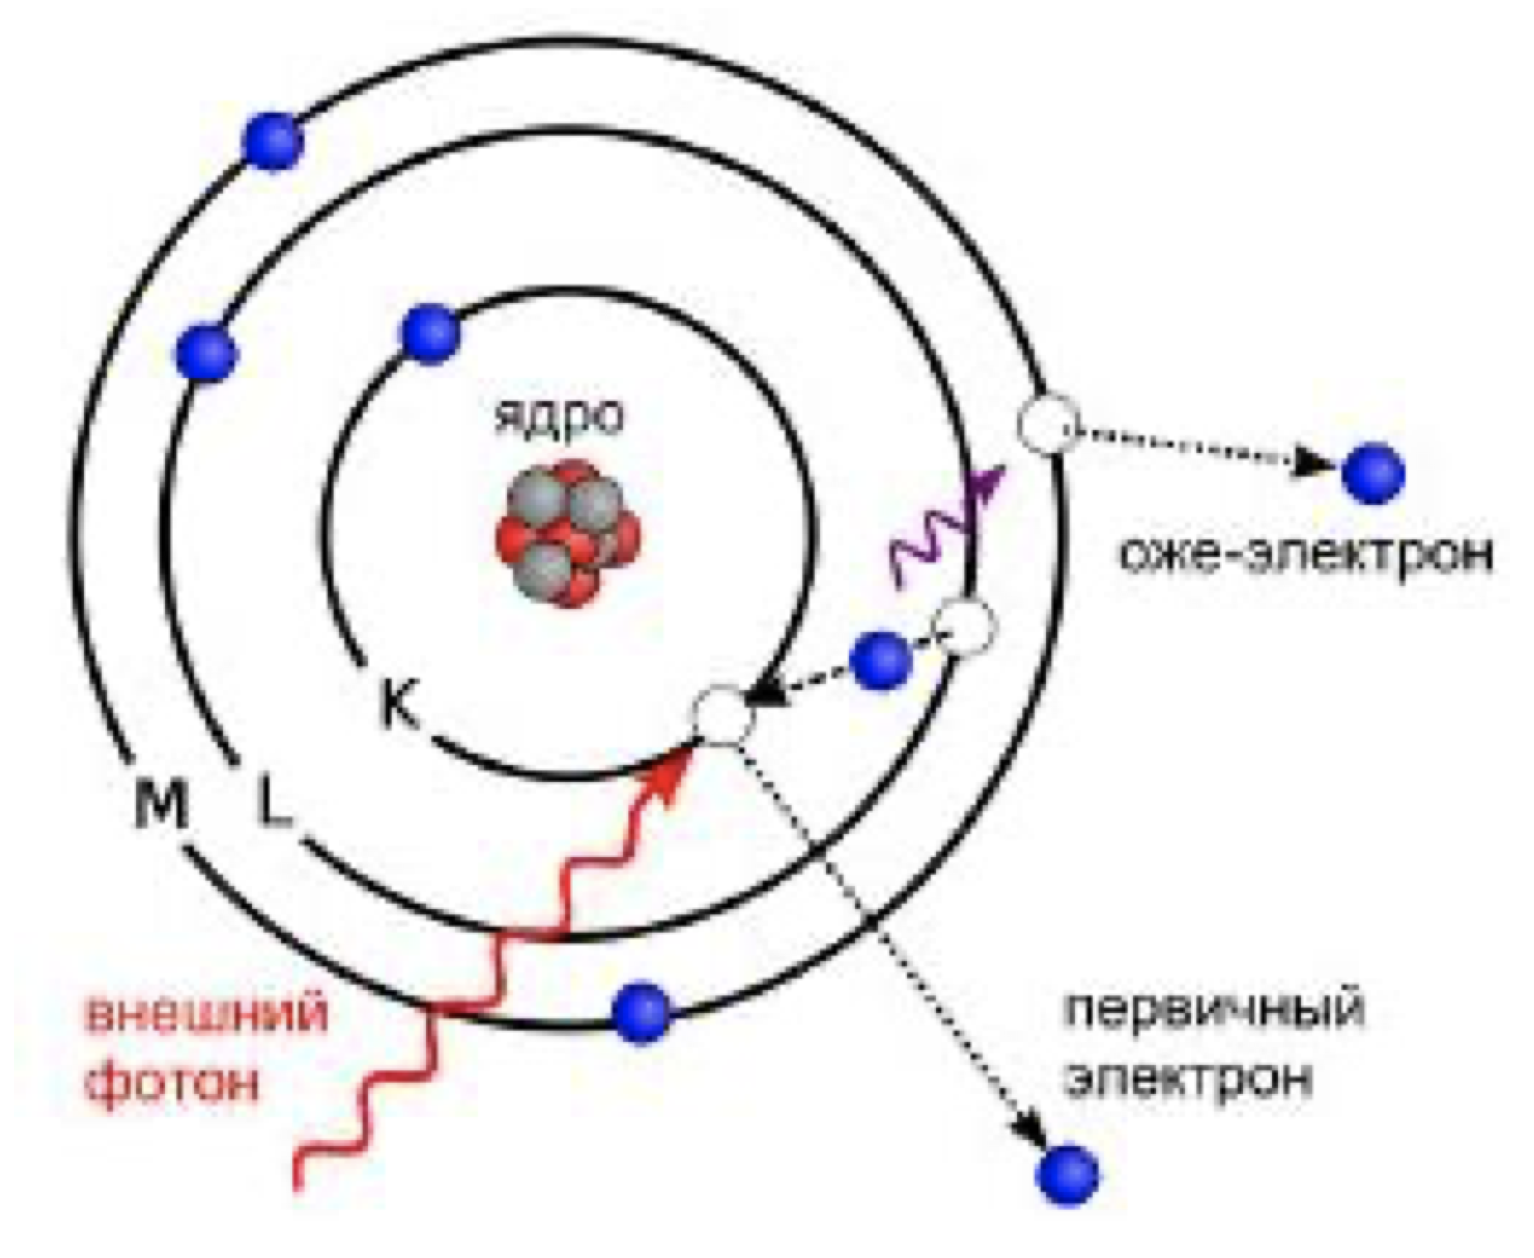
\includegraphics[scale = 0.5]{oge.png}
            \caption{Оже-генерация}
        \end{center}
    \end{figure}

    \item \textbf{Почему длина экранирования локального пространственного заряда в металле на порядки меньше, чем в полупроводнике?} \par 
    \textit{Дебавеская длина} - расстояние, на которое распространяется действие электрического поля отдельного заряда в квазинейтральной среде, содержащей свободные положительно и отрицательно заряженные частицы. 
    $$\lambda_D = \left( \sum_j \frac{4 \pi q_j^2 n_j}{\varepsilon_rkT_j} \right)^{-1/2}$$
    Длинна экранирования обратно пропорциональна концентрации носителей зарядов, в металле количество электронов проводимости значительно больше чем в полупровднике, поэтому длина экранирования металлов меньше.

    \item \textbf{Почему при оценке быстродействия фотодиода не учитывается время перемещения вылетевшего из области пространственного заряда (ОПЗ) основного фотоносителя по нейтральной области до токового контакта?} \par 
    Быстродействие фотодиодов определяется рекомбинацией дополнительных носителей заряда. Обычно толщина области, на которою падает излучение, больше или порядка 1/$\alpha$, где $\alpha$ — коэффициент поглощения, и меньше диффузионной длины неосновных носителей заряда. 
    В этом случае быстродействие определяется отношением толщины этой области к диффузионной длине и может быть значительно меньше времени жизни неравновесных носителей заряда.

    \item \textbf{Проиллюстрировать с помощью зонной диаграммы в E – p пространстве, что электрон и дырка уменьшают свою энергию в зоне проводимости и в валентной зоне.} \par 
    \begin{figure}[H]
        \begin{center}
            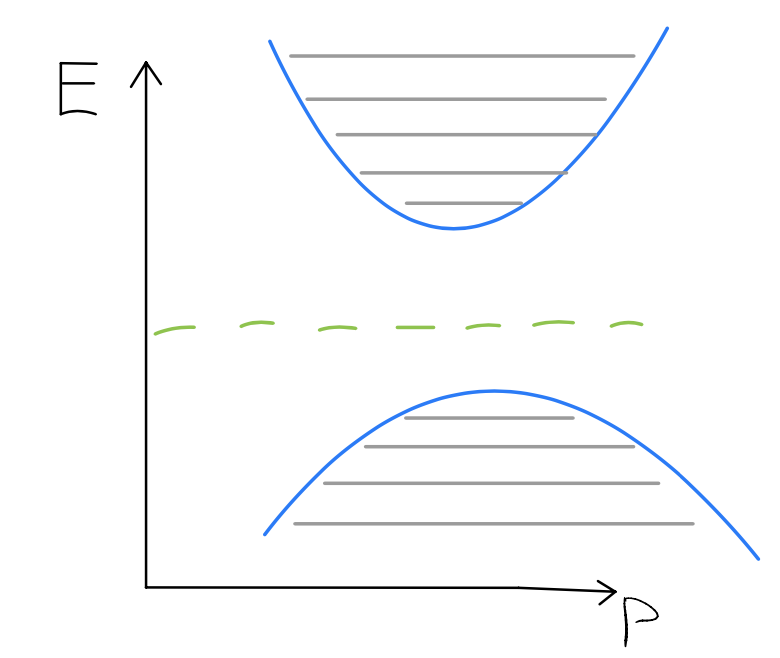
\includegraphics[scale=0.4]{p1.png}
        \end{center}
    \end{figure}

\end{enumerate}


\end{document}